

\subsubsection{Volume}

The next quantity is volume. Its representation as a time series is:

\begin{figure}[H]
    \centering
    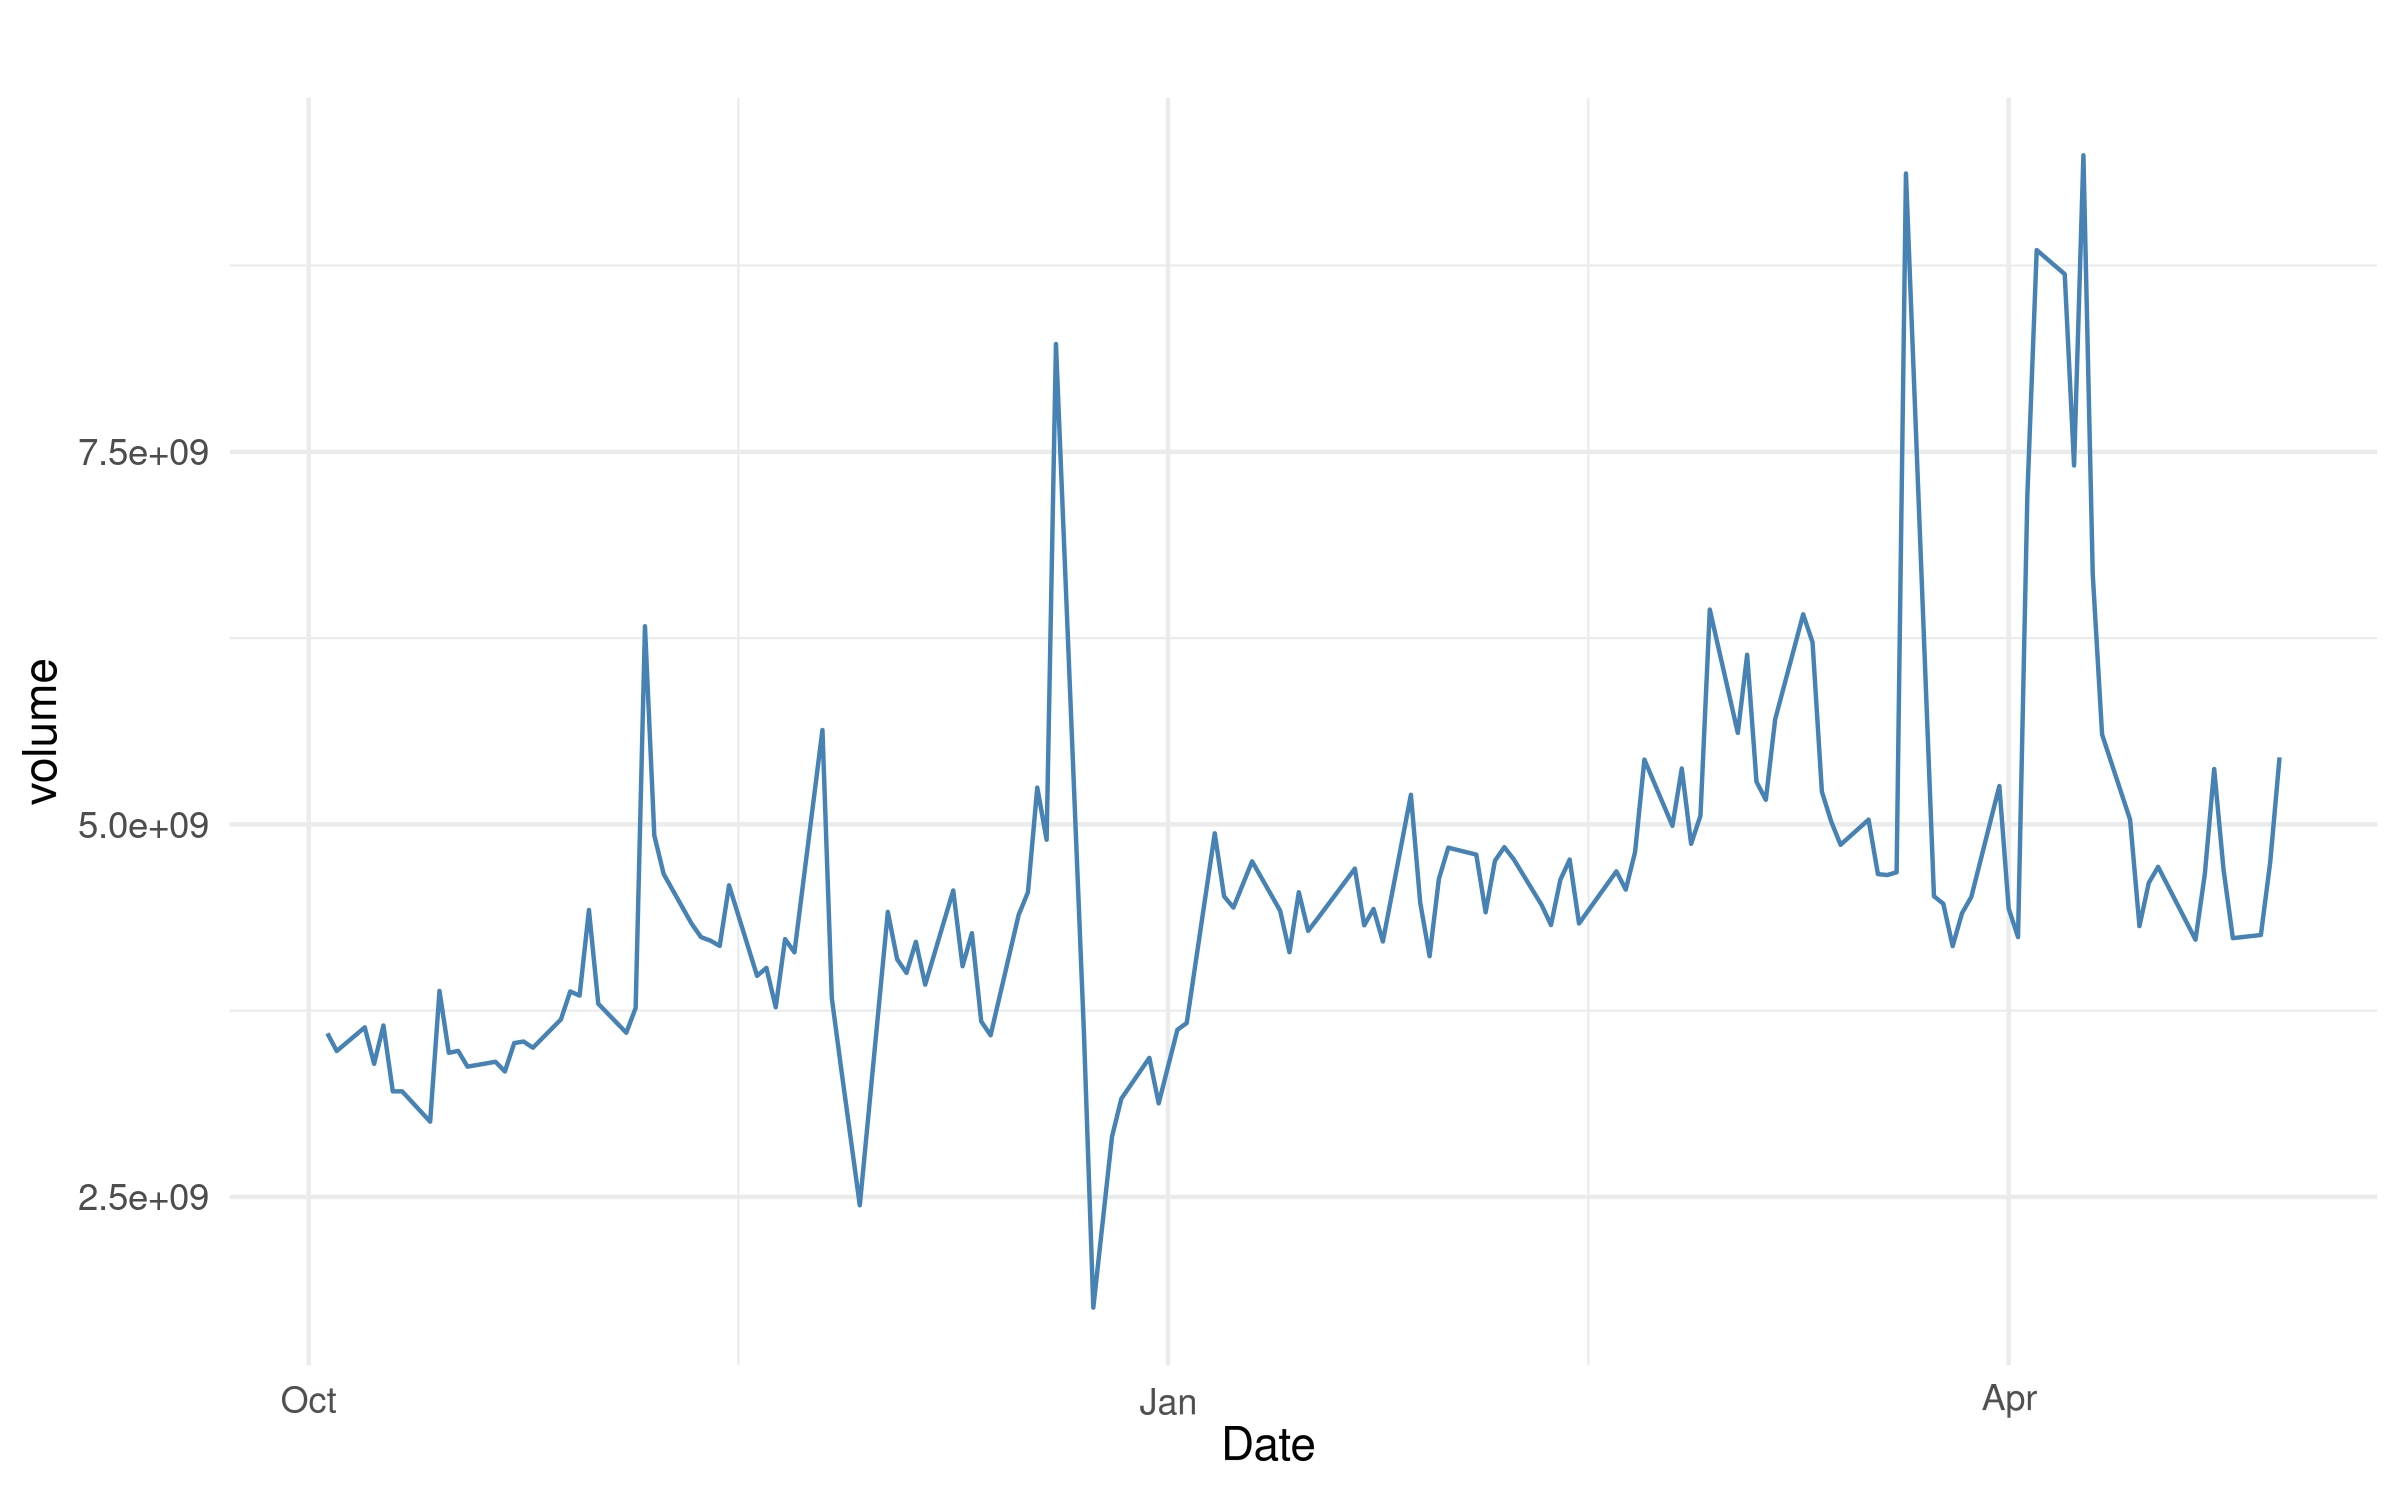
\includegraphics[width=0.8\textwidth]{../pavic_r/volumen_timeseries.png}
    \caption{m during the period examined}
    \label{fig:hml_timeseries}
\end{figure}

The five-number summary is:

\begin{align*}
(x_0(v), q_L(v), m(v), q_U(v), x_{(n)}(v)) &= (1757720000,\; 3880610000,\; 4432250000,\; 4866380000,\; 9489600000)    
\end{align*}

A natural question is which distribution the volume of a trading day comes from. To investigate this further, we plotted its histogram and the histogram of its logarithm. This produced the following plots:

\begin{figure}[H]
    \centering
    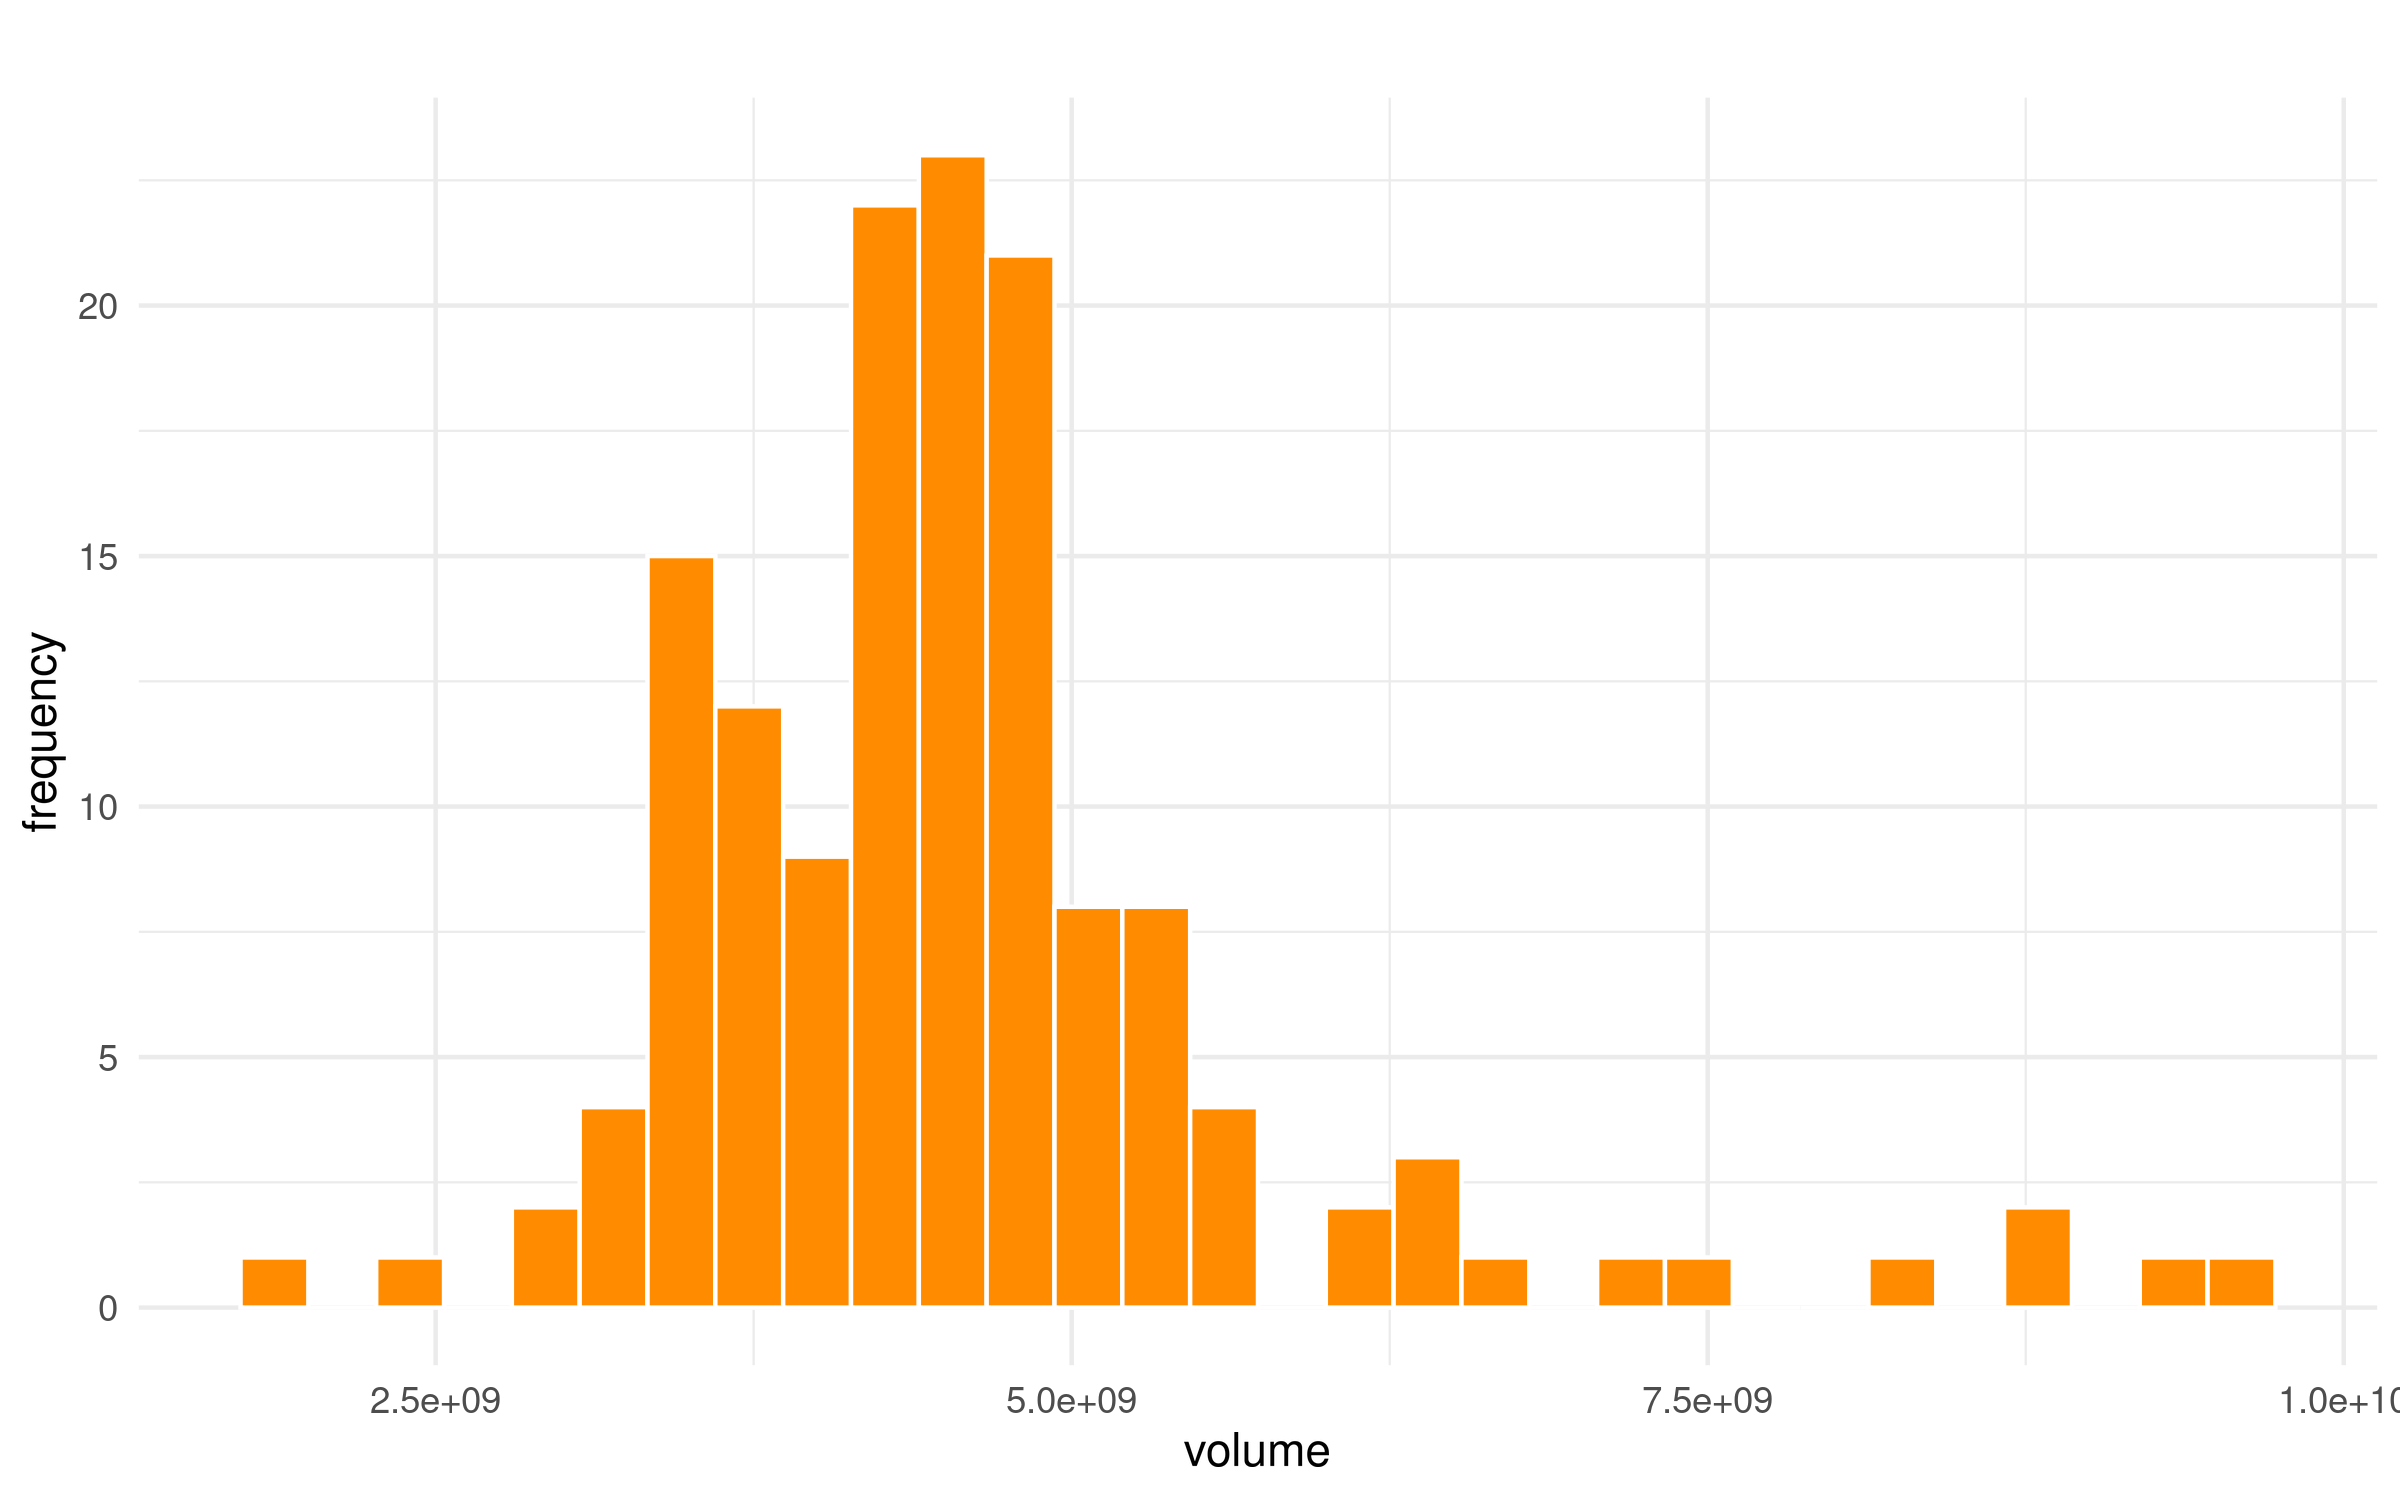
\includegraphics[width=0.8\textwidth]{../pavic_r/volumen_histogram.png}
    \caption{Histogram of volatility during the period examined}
    \label{fig:volumen_histogram}
\end{figure}

\begin{figure}[H]
    \centering
    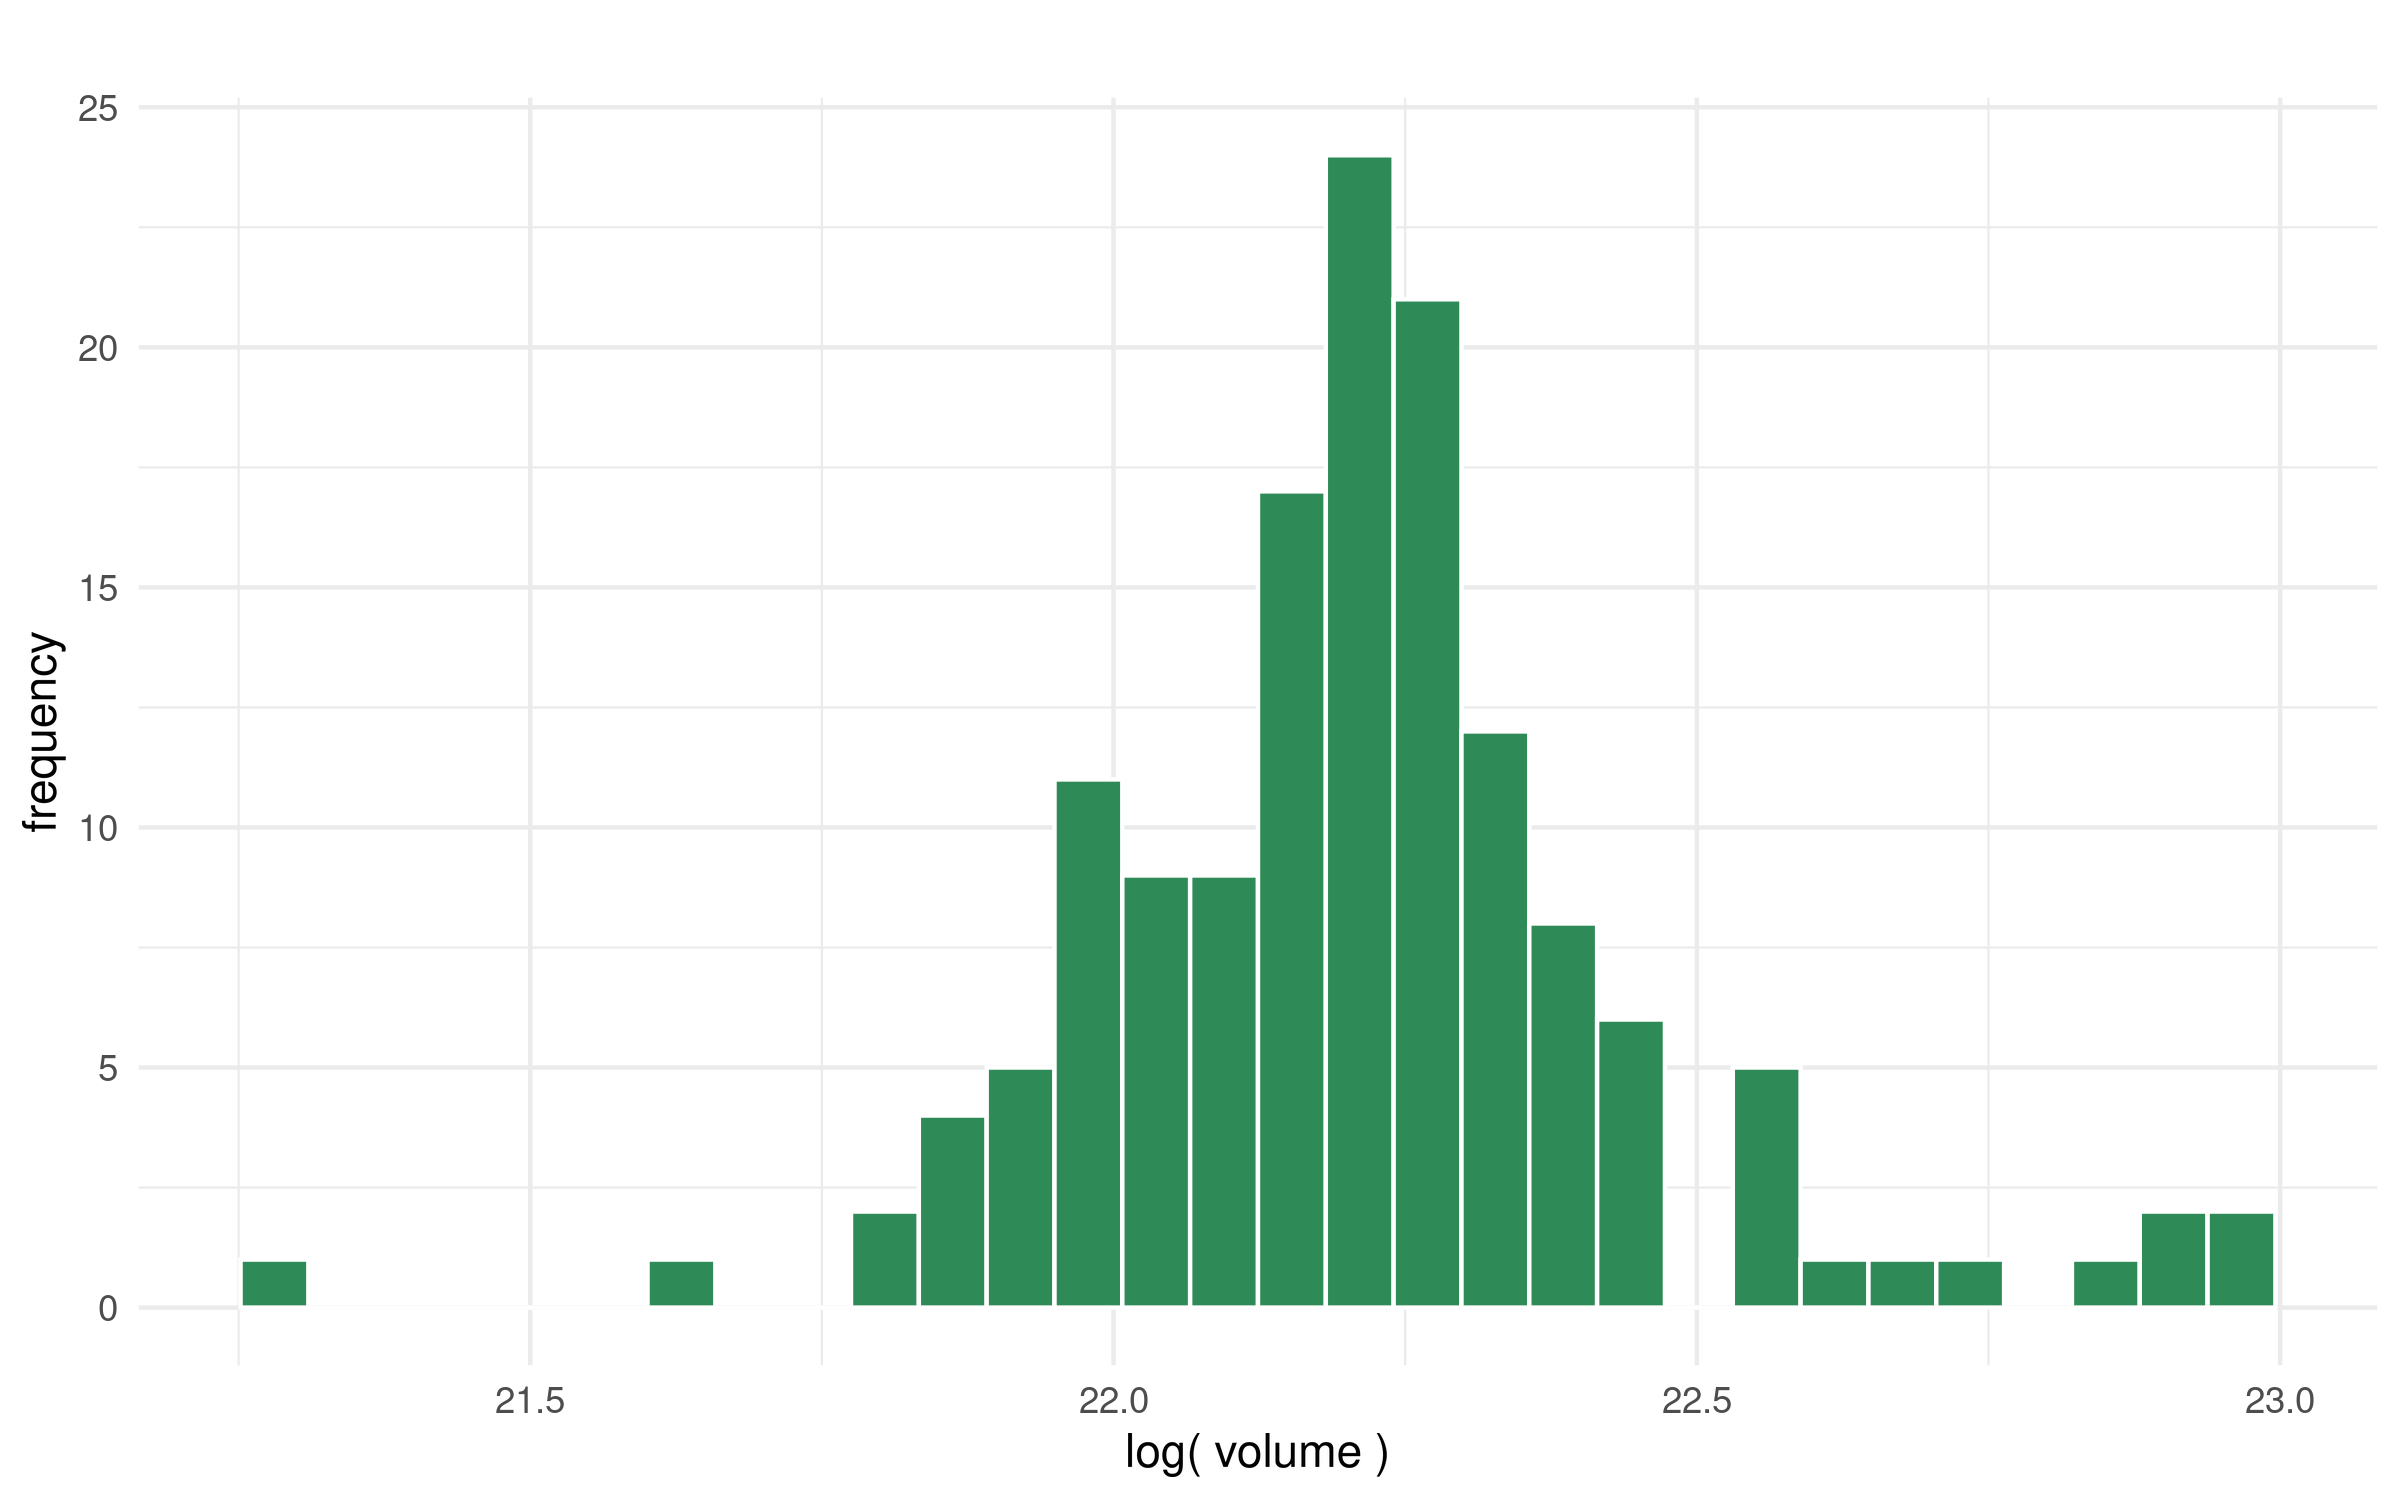
\includegraphics[width=0.8\textwidth]{../pavic_r/volumen_loghistogram.png}
    \caption{Histogram of log(volatility) during the period examined}
    \label{fig:volumen_loghistogram}
\end{figure}

\subsubsection{Change}

The final quantity is change. It was calculated using the formula

\[ \text{change} = (\,\text{opening price}\,) - (\,\text{closing price}
\,) \]

Its representation as a time series is:

\begin{figure}[H]
    \centering
    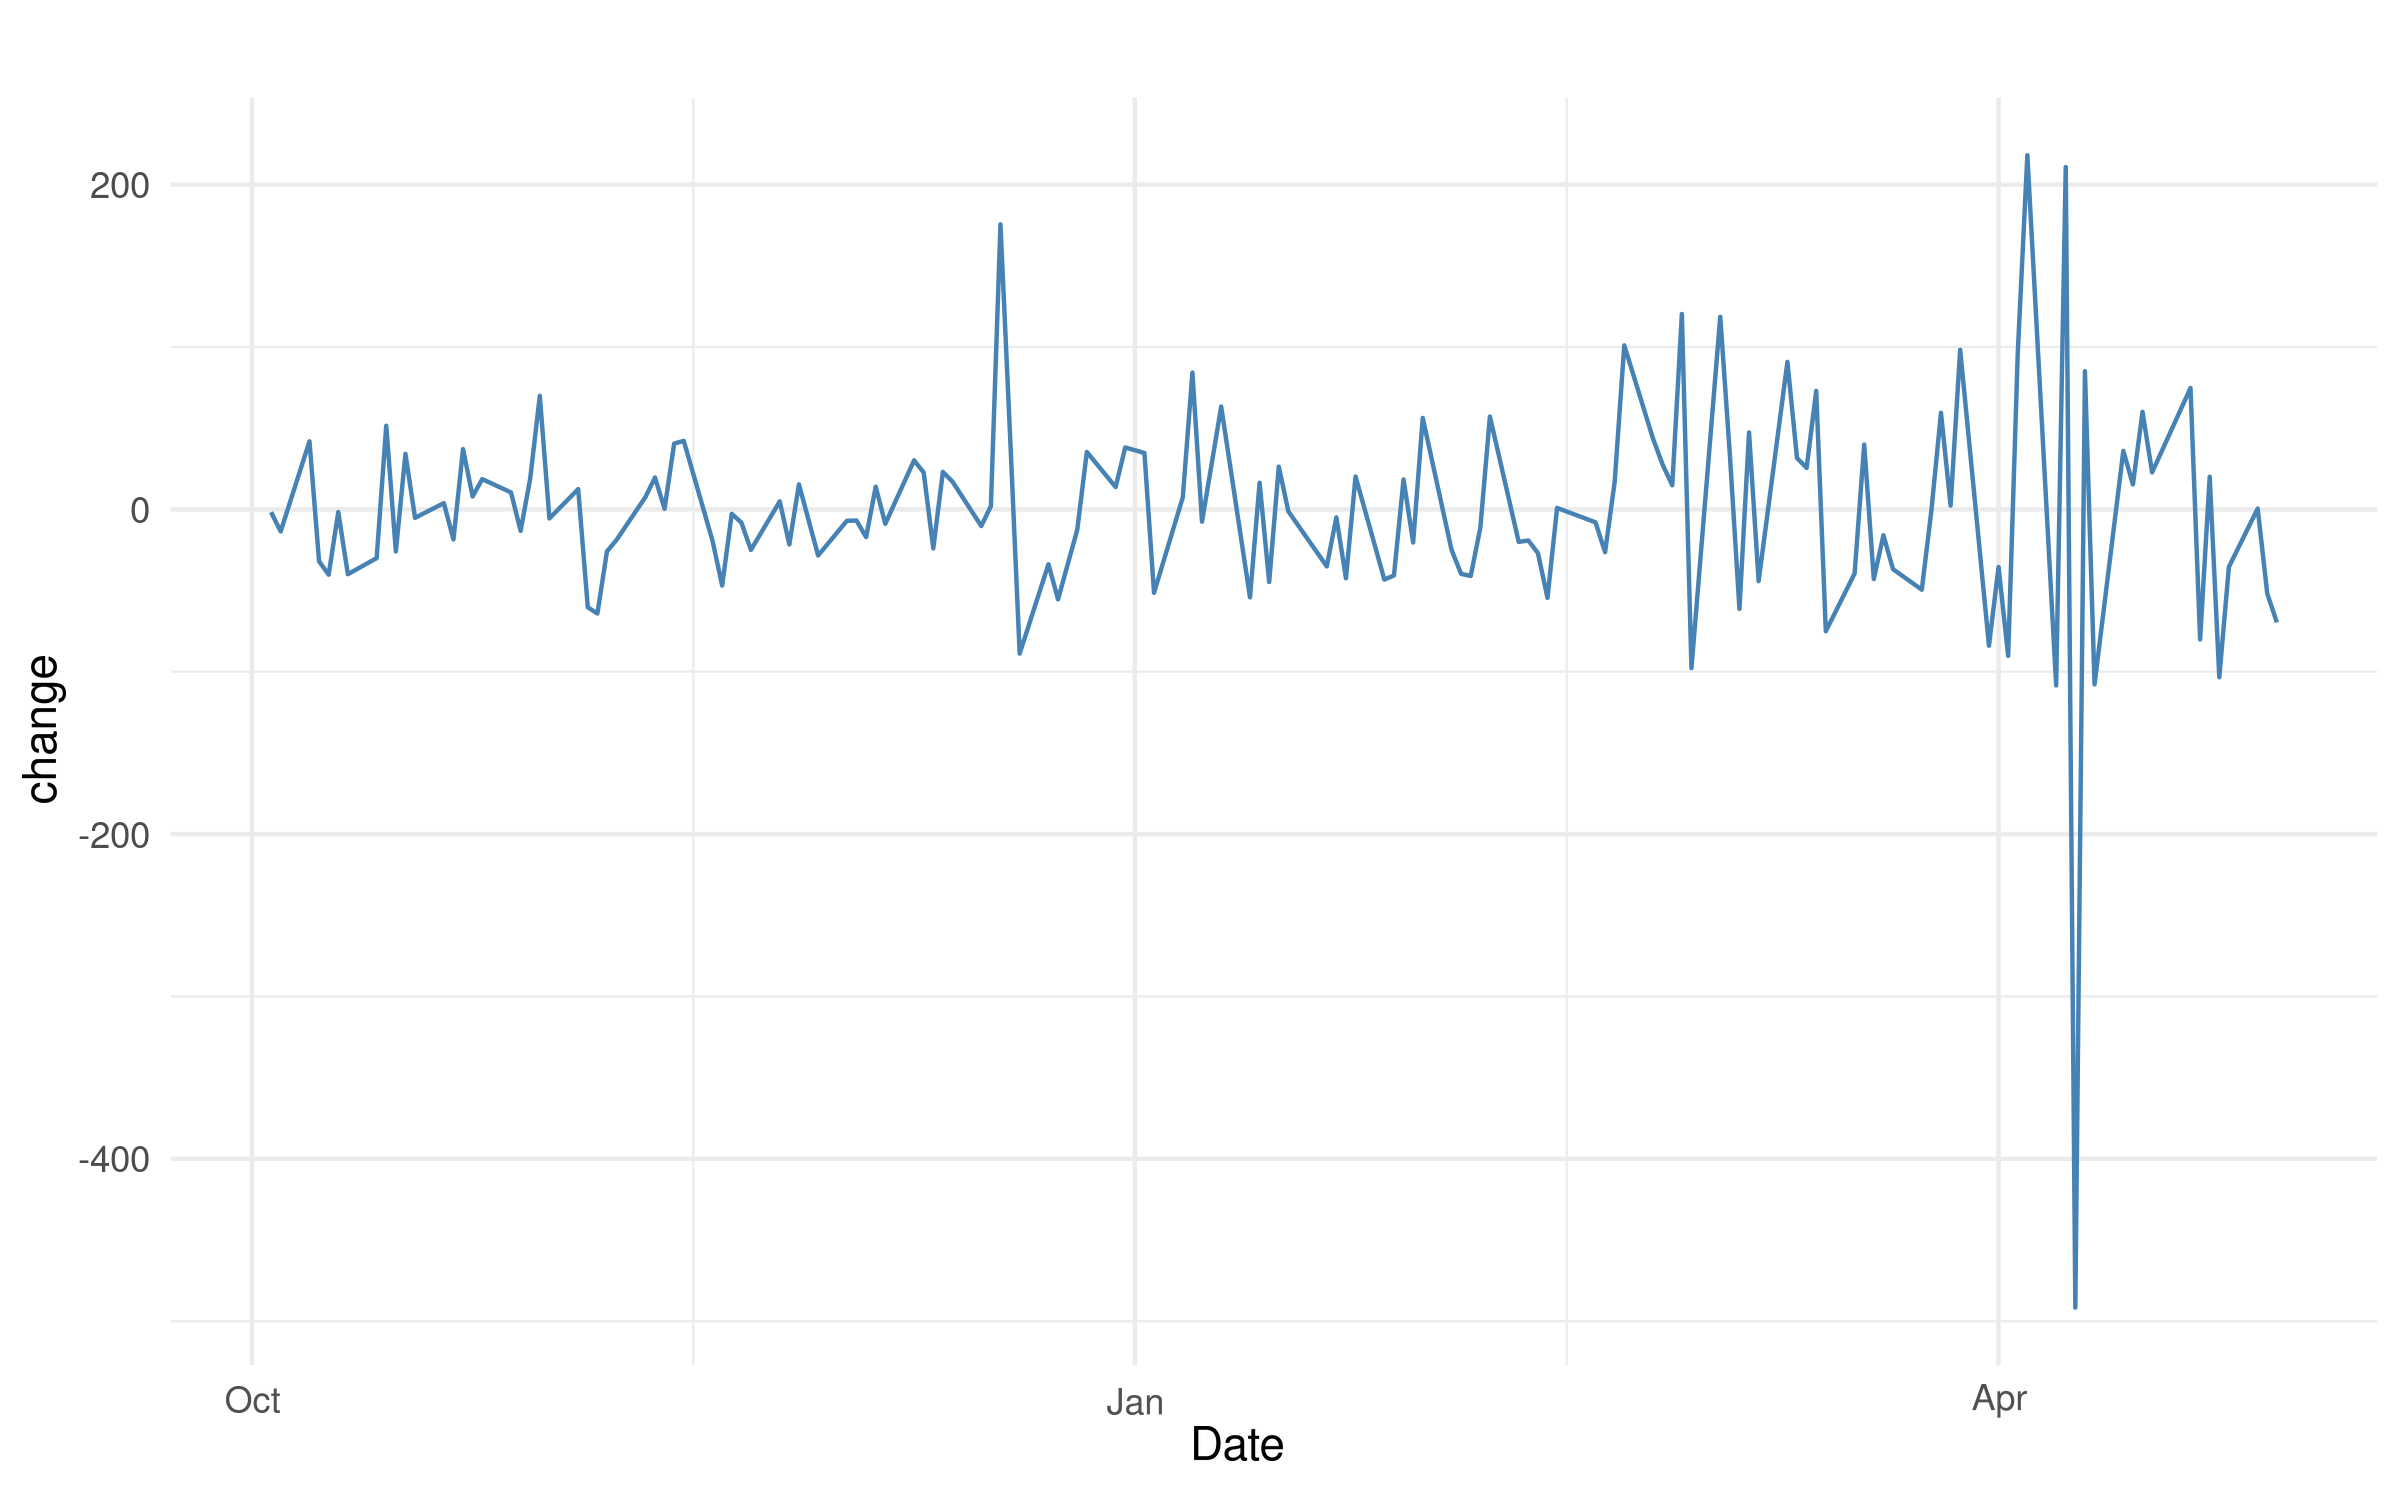
\includegraphics[width=0.8\textwidth]{../pavic_r/promjena_timeseries.png}
    \caption{Volatility during the period examined}
    \label{fig:promjena_timeseries}
\end{figure}

The five-number summary is:

\begin{align*}
(x_0(v), q_L(v), m(v), q_U(v), x_{(n)}(v)) &= (-491.62012,\; -34.46997,\; -1.75000,\; 28.81982,\; 218.06006)    
\end{align*}

A natural question is which distribution the price change of a trading day comes from. To investigate this further, we plotted its histogram and the histogram of its logarithm. This produced the following plots:

\begin{figure}[H]
    \centering
    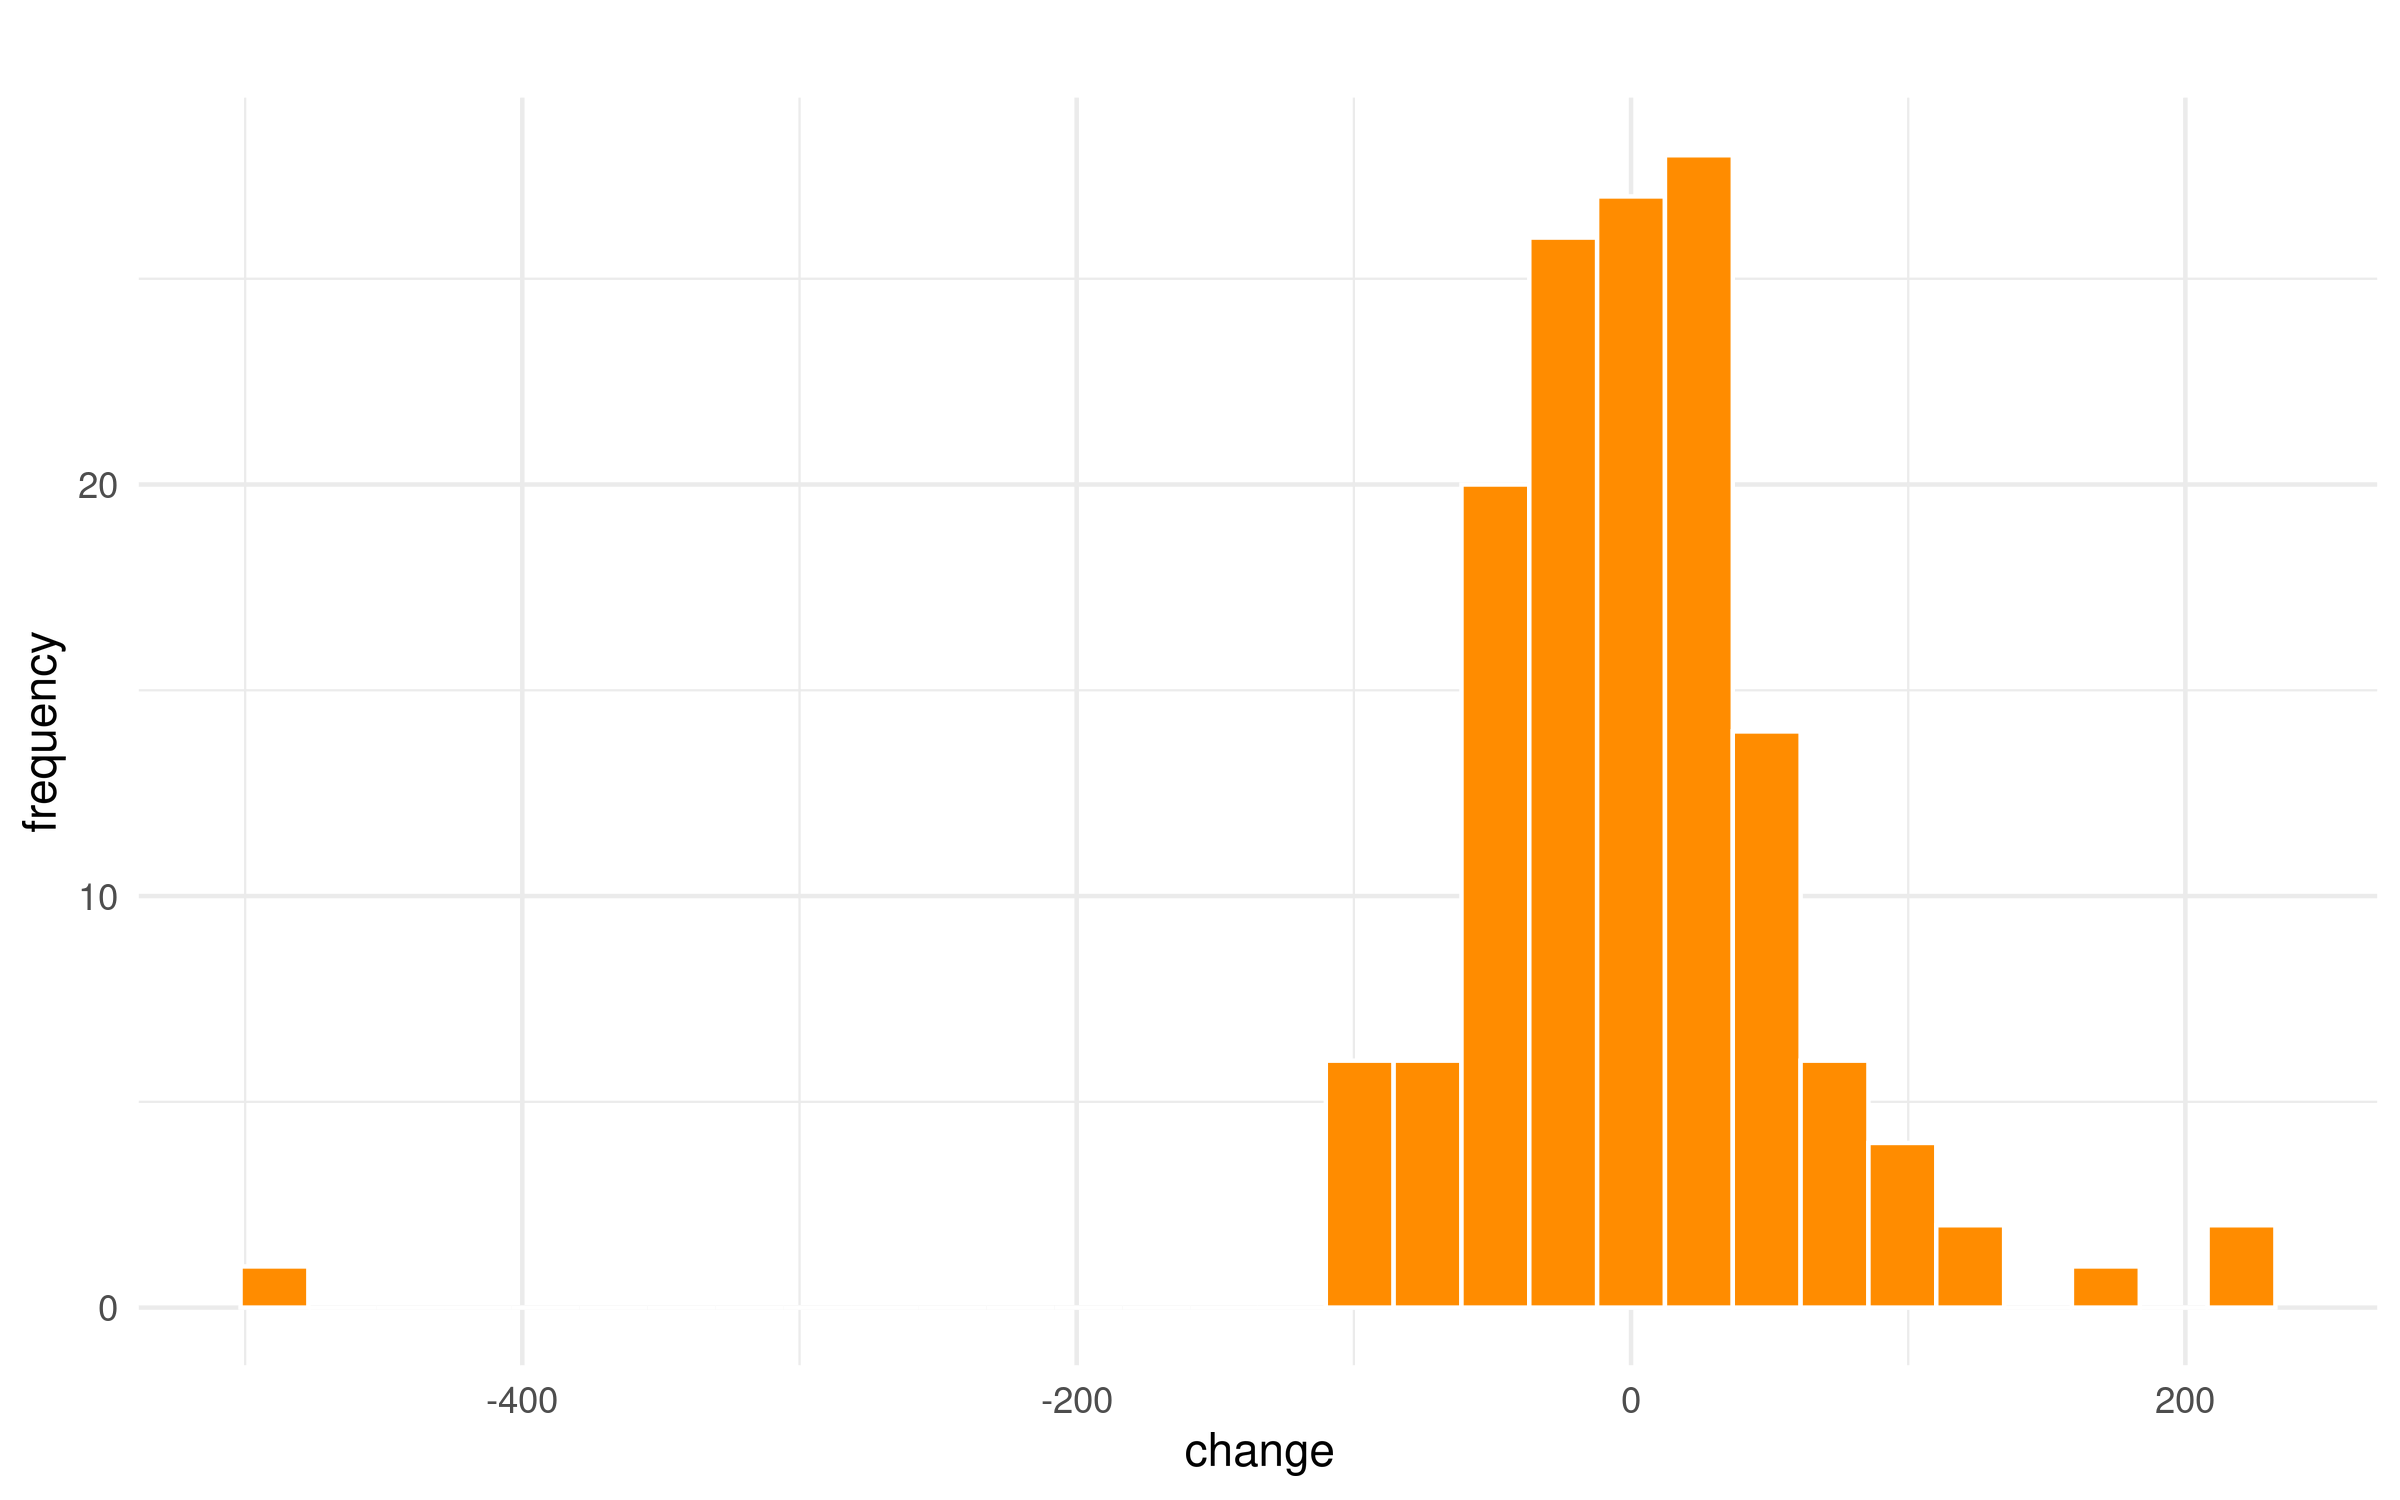
\includegraphics[width=0.8\textwidth]{../pavic_r/promjena_histogram.png}
    \caption{Histogram of volatility during the period examined}
    \label{fig:promjena_histogram}
\end{figure}

\begin{figure}[H]
    \centering
    \includegraphics[width=0.8\textwidth]{../pavic_r/promjena_loghistogram.png}
    \caption{Histogram of log(volatility) during the period examined}
    \label{fig:promjena_loghistogram}
\end{figure}

\end{document}